At the highest level, our game can be broken into 5 major systems that will work 
together to provide the experience we are hoping to create. These parts are The 
Engine, The Puzzle System, The User Interface, The Interpreter, and The Actor. 
The relationship between these systems has been designed to be as simple as 
possible. As shown in Figure \ref{fig:overall_system_diagram}, each major system 
is only responsible for interfacing with two others. 

\begin{figure}[!hb]
    \caption{Computron System Overview}
    \label{fig:overall_system_diagram}
    \centering
    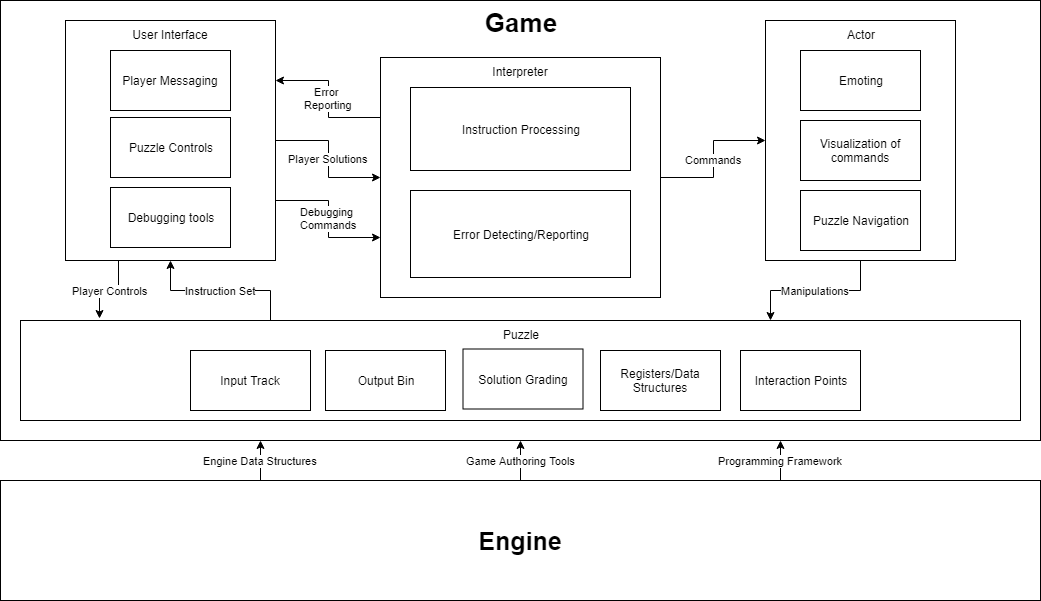
\includegraphics[width=\textwidth]{Diagrams/SystemDiagram.png}
\end{figure}

The nature of these interfaces, as well as the operations, responsibilities, and 
requirements of each of these major systems, will be detailed in the subsequent sections.